\documentclass[smallextended]{svjour3}
\usepackage[utf8]{inputenc}
\usepackage{amsmath,amsfonts,amssymb,color,hyperref}
\usepackage{lmodern}
\usepackage{amssymb}
\usepackage{amscd}
\usepackage{latexsym}
\usepackage{graphicx}
\usepackage{bm}
\usepackage{float}
\usepackage{mathrsfs}
\usepackage{subfigure}
\usepackage{xargs}
\usepackage[pdftex, dvipsnames]{xcolor}
\usepackage[colorinlistoftodos, prependcaption, textsize=tiny]{todonotes}
\newcounter{chapter} % to fix the bug in svjour3
\usepackage{cleveref}
\usepackage[round]{natbib}
\usepackage{tikz}
\usepackage{tikz-3dplot}
\usepackage{pgfplots}
\usepackage{siunitx}
\pgfplotsset{compat=newest}
\usepgfplotslibrary{smithchart}
\usetikzlibrary{pgfplots.units}

\bibliographystyle{abbrvnat}
%==============================================================================
\newcommandx{\unsure}[2][1=]{
        \todo[linecolor=red,
                backgroundcolor=red!25,
                bordercolor=red, #1]{#2}
        }
\newcommandx{\change}[2][1=]{
        \todo[linecolor=blue,
                backgroundcolor=blue!25,
                bordercolor=blue, #1
        ]{#2}
        }
\newcommandx{\info}[2][1=]{
        \todo[
            linecolor=OliveGreen,
            backgroundcolor=OliveGreen!25,
            bordercolor=OliveGreen, #1]{#2}
     }
\newcommandx{\improvement}[2][1=]{
        \todo[linecolor=Plum,
                backgroundcolor=Plum!25,
                bordercolor=Plum,#1]{#2}
    }
\newcommandx{\thiswillnotshow}[2][1=]{
                \todo[disable,#1]{#2}
            }
%
\newcommand{\cqd}{\hfill$\Box$}
\newcommand{\f}{{\mathcal F}}
\newcommand{\IR}{{\mathbb R}}
\newcommand{\R}{{\mathbb R}}
\newcommand{\IN}{{\mathbb N}}
\newcommand{\ind}{\mbox{\Large$\chi$}}
\newcommand{\tor}{{\mathbb T}}
\newcommand{\G}{{\mathbb G}}
\newcommand{\beq}{\begin{equation}}
\newcommand{\eeq}{\end{equation}}
\newcommand{\bal}{\begin{align}}
\newcommand{\eal}{\end{align}}
\newcommand{\beqn}{\begin{equation*}}
\newcommand{\eeqn}{\end{equation*}}
\newcommand{\baln}{\begin{align*}}
\newcommand{\ealn}{\end{align*}}
\newcommand{\tbar}{\bar t}
\newcommand{\xbar}{\bar x}
\newcommand{\ep}{\epsilon}
\newcommand{\Pb}{\mathbb P}
\newcommand{\Rl}{\mathbb R}
\newcommand{\E}{\mathbb{E}}
\newcommand{\tf}{\mathcal{F}}
\newcommand{\hac}{\mathcal{H}}
\newcommand{\hact}{\mathcal{H}_T}
\DeclareMathOperator{\Var}{Var}
%
%
%
\begin{document}
%
    \title{A stochastic model of mortality rate with memory}
    \subtitle{A stochastic model of mortality rate with memory}
    \author{Francisco Delgado-Vences 
        \and
        Arelly Ornelas
        \and
        Saul Diaz-Infante
    }
%
    \institute{
        Francisco Delgado-Vences
        \at
        Conacyt-Universidad Nacional Aut\'onoma de \'Mexico.
        \\
        Instituto de Matem\'aticas, Oaxaca, M\'exico
        \\
        \email{delgado@im.unam.mx}
        \\
        ORCID:
        \and
        %
        Arelly Ornelas
        \at
        Conacyt-Instituto Politecnico Nacional-CICIMAR,
        \\
        La Paz, M\'exico
        \\
        \email{arelly.ornelas@conacyt.mx}
        \\
        ORCID:
        \and
        %
        Saul Diaz-Infante
        \at
        Conacyt-Universidad de Sonora
        \\
        Departamento de Matemáticas,
        \\
        Hermosillo, Sonoran M\'exico
        \email{sdinfante@conacyt.mx}
        \\
        ORCID: 0000-0001-9559-1293
    }
    \date{Received: \today / Accepted: date}
    \maketitle
%
    \begin{abstract}
            An accurate estimation of mortality rates is essential to make
        decisions. For example, the ensures companies, banks, 
        among others, plans its operations according to estimations  based 
        on  these rates. However, the vast number of variables and its 
        intricate relation implies a challenge for the estimation of these 
        rates.
    
            We assume the following hypothesis: the mortality rate has a strong
        relationship with its owns past. In this line, we propose a stochastic
        model with long-term memory that describes mortality. Then, using data 
        from Italy, we provide statistical evidence via Hurst parameter 
        estimation that does not reject our hypothesis. Further, we extract a 
        subset of data to evaluate its forecasting performance, and we observe 
        a good estimation.
    
            To the best of our knowledge, our contribution is the first attempt
        that includes long term memory in the formulation of a model to
        describe mortality rates. Our results suggest that the hypothesis of an
        imperfect correlation intensity across generations would be more 
        realistic.
    \end{abstract}
%
%
\section{Introduction} \label{intro}

        Future planning in the demographic, economic, and actuarial areas is
    crucial. For instance, proper planning in social programs, government
    budgets, cost of insurance, and others depends on the forecast. However,
    constant changes in technology, lifestyle, migration, to name a few, make
    predicting a demanding task.  Mortality impacts directly in cash and
    therefore need a reliable future projection.

        Previous work has only focused on deterministic or stochastic models
    without memory effects. \cite{pitacco2009modelling} review 
    the first mortality tables and models.
    \cite{mi-pr} report a linear SDE driven by Brownian motion that describes
    the mortality hazard rate. In \cite{gi-or-be}, the authors extend the
    Mikevesky model to an SDE with time-dependent diffusion and study a type of
    autoregressive model for the logarithm of the hazard rate.   
    \cite{je-lu-vi} formulate a cohort-based model with imperfect correlation
    across generations and use data from UK to estimate parameters.

        This paper aims to show statistical evidence that mortality rates
    follow a stochastic process with long-range dependence (LRD), that is,
    a stochastic process with memory. According to \cite{ra}, a stochastic
    process or time series is LRD, if it has persistence behavior\textemdash
    below we give a formal definition.

        We base our stochastic formulation in the fractional Brownian Motion 
    (fBM) \citep[see ]{ma-va}. Since fBM is a generalization of the standard 
    Brownian Motion (BM) that still satisfies self-similarity and is LRD, fBM 
    results to be a natural noise model to describe LRD behavior.

        The main idea is to extend the stochastic model reported by 
    Milevesky and Promislow to a model with LRD and verify its performance 
    to fitting and forecasting with real data.  

        We obtain statistical evidence\textemdash via Hurst parameter 
    estimation\textemdash that Italy mortality rate data is LRD. Our model 
    captures women's mortality rate dynamics. But we observe that the Italian
    man has a higher mortality rate and variance. These results suggest 
    that stratification by gender would be a direction for future formulations.
   
       
        Our work exhorts to explore the long time memory effects of dynamics 
    under uncertainty. Also these ideas could improve mathematical models, 
    which considers mortality in its formulation, for example, models for 
    infectious  disease spread or population growth.
    

        After this brief introduction, we formulate our fractional model in 
    \Cref{model-form}. \Cref{fgn} reviews the fBM and presents
    the fractional Ornstein-Uhlenbeck (fOU) process. \Cref{esti} outlines the
    applied method for parameter estimation. In  \Cref{re-fou}, we implement our
    formulation to fitting data of mortality from Italy. Further, in
    this section, we also run forecasting to a subset of the data and evaluate
    its efficiency. Finally, we conclude in \Cref{sec:Conclutions}.

\section{Model formulation}\label{model-form}
       Our formulation relies on the model of \cite{mi-pr}, bellow we review 
    the main ideas.
    
        Let $Y_t$ the solution process to the stochastic differential equation 
    driven by standard Brownian motion.
    \begin{equation} \label{mod-3}
        \begin{aligned}
            dY_t  = & -\lambda Y_t dt + \sigma dB_t,
            \\
            & \lambda, \sigma > 0, \ Y_0 = 0, \ t \in [t_0,T] .
        \end{aligned}
    \end{equation}
        According to the Milevsky-Promislow model, $h_x$ denotes the 
    stochastic force of mortality at time t of an individual aged $x$. Letting 
    $h_x(t) = h(t)$, and conforming  with SDE \eqref{mod-3}, this ratio is 
    described by 
    \begin{equation}
        \label{eqn:mortality_hazard_rate}
        \begin{aligned}
            h(t)  = & h_0
                \exp(\alpha_0t + \alpha_1 Y_t)
            \\
            & h_0, \alpha_0, \alpha > 0.
        \end{aligned}
    \end{equation}
     Next, the survival probability of an individual aged $x$ in the period 
    $[t,T]$ as
    \begin{equation}\label{E-surv}
        S(t,T):=
            \E
            \Big[
                \exp\Big(
                    -\int_t^T h_x(u) du
                    \Big)
                \Big|\mathcal{F}_t 
            \Big],
    \end{equation}
    where $\{\mathcal{F}_t\}_{t\ge 0} $ is a filtration which represent the 
    information until time $t$.

        Our formulation extends the Milevsky model 
    \cref{mod-3,eqn:mortality_hazard_rate,E-surv} by utilizing  fractional 
    Brownian motion. That is, instead of the Ornstein–Uhlenbeck process 
    (OU) defined by SDE \eqref{mod-3}, we employ its fractional version
    (fOU)
    \begin{equation}
        \label{mod2}
        \begin{aligned}
            dY_t^H & 
                =
                - \lambda Y_t ^ H dt 
                + \sigma dB_t ^ H, 
                \\
                 & \lambda, \sigma > 0,
                  \ Y_0 = 0,
                  \ H \in [1 / 2, 1) .
        \end{aligned}
    \end{equation}
    In fact we implement the integral form of the above fractional SDE
    \begin{align}
        \label{mod3}
        Y_t ^ H & =
            - \lambda
            \int_0 ^ t 
                Y_s ^ H ds 
                + 
                \sigma B_t ^ H.
    \end{align}
    fOU process is long time-dependent when $H \in [1/2,1)$ 
    \citep[for details see][]{ch-ka-ma,Anh2002,Hu2005,Kleptsyna2002}. Then, we 
    use the fOU to explore the long time dependence of mortality hazard-rates.


\section{Fractional Gaussian processes} \label{fgn}
    \subsection{Fractional Brownian motion} \label{fBm}
        \todo{Introductory paragraph}
        We consider the Gaussian process$\{B_t^H,t\ge 0\}$, with $H\in (0,1)$,
    zero-mean and covariance function given by
    \begin{align}
        R_H(t,s):=
            \E(
                B_s^H B_t^H
            )
            =
            \tfrac{1}{2}
            \big(
                t ^ {2 H} + s ^ {2 H}
                - |t - s| ^ {2 H}
            \big).\label{s1.1}
    \end{align}
%

        This stochastic process is the so called 
    \emph{fractional Brownian motion} (fBM). 
    \citeauthor{ko} introduced this fractional process 
    in 1940 and \citeauthor{ma-va} gives an in-depth study in 1968.
    The parameter $H$ is called Hurst index in honor to the statistical 
    analysis developed by the climatologist Harold Edwin Hurst. 
    
        The fBm is a generalization of Brownian motion without independent 
    increments, in fact,  it is a continuous-time Gaussian process wich
    has the properties of self-similarity and stationary increments. Its 
    sample-paths are almost nowhere differentiable and
    almost-all H\"{o}lder continuous for any order strictly less than $H$. That 
    is, for each trajectory, there exists a finite constant $C$ such that for 
    every$\epsilon > 0$
    \[
        \E \big(
            | B_t ^ H - B_s ^ H|
        \big)
        \le
        C |t - s| ^ {H - \epsilon} .
    \]
%
    For $H = \tfrac{1}{2} $, the covariance of fBM follows
    $
        R_{1 / 2} (t, s)
            = \min(s, t)
    $, thus process $B_t ^ {1 / 2}$, is equivalent to
    the standard Brownian motion. However, if $H \ne \tfrac{1}{2}$, 
    then this increments are dependent.
%
        Let  $X_n = B_n ^ H - B_{n - 1} ^ H$, $n \ge 1$.
    Then $\{X_n, n \ge 1\}$ is a Gaussian stationary sequence with unit
    variance and covariance function 
    \begin{align*}
        \rho_H (n) &=
            \frac{1}{2}
            \Big(
                (n + 1) ^ {2 H} + (n - 1) ^ {2 H}
                - (2 n) ^{2 H}
            \Big)
            \\
            &\approx
            H (2H - 1)n^{2H-2} \to 0, \quad n \to \infty.
    \end{align*}
    Therefore,
    \begin{itemize}
        \item
            if $H > \tfrac{1}{2}$, then $\rho_H(n) > 0$ for $n$ large enough and
            $\sum_{n=1}^\infty \rho_H(n)=\infty$. In this case, we say that
            process $X_n$ is persistent with positive correlation and that
            $X_n$ has the \emph{long-range dependence} property
        \item
            if $H < \tfrac{1}{2}$, then $\rho_H(n) < 0$ for $n$ large enough and
            $\sum_{n=1}^\infty \rho_H(n)<\infty$. Thus we say that $X_n$ is an 
            anti-persistent process with negative correlation.
    \end{itemize}
    For further information on fBM see \cite{ra,nu,mi}.
    
    \subsection{The Fractional Ornstein-Uhlenbeck process}\label{sect-OU}
        The fOU is an SDE driven by a fractional Brownian motion. 
    Coming back to Equation \eqref{mod3}, \cite{ch-ka-ma}
    introduced the fractional Ornstein-Uhlenbeck process (fOU) and they 
    showed that the process
    \begin{equation}
        Y_t ^ H = 
            \sigma \int_0 ^ t e ^ {-\lambda(t - u)} dB_u^H, 
        \label{mod4}
    \end{equation}
    is the unique almost surely continuous-path process which solves 
    \eqref{mod3} (see also Theorem 1.24 in \cite{ra}).
    The integral in Equation \eqref{mod4} is a
    pathwise Riemann–Stieltjes integral.  The fOU process is neither Markovian 
    nor a semimartingale for $H \in(1/2,1)$  \citep[see][]{du-no} but remains
    Gaussian and ergodic. Moreover, when $H \in(1/2,1)$, $Y_t$ has the 
    long-range dependence property \cite{ch-ka-ma,ra}.

    According to \cite{ze-ch-ya}, the variance of the fOU process $Y_t$ is 
    given by the following expression:
    \begin{align}
        \Var(Y_t)= 
            \sigma^2 2H e^{-2\lambda t} 
            \int_0^t s^{2H-1} e^{2\lambda s} ds.\label{var-fou}
    \end{align}
    Notice that when $H=1/2$ we get
    \begin{align}
        \Var(Y_t)= \frac{\sigma^2}{2\lambda}  \big(1-e^{-2\lambda t}\big),
    \end{align}
    which is the variance of the standard Ornstein-Uhlenbeck process 
   \citep[see][p. 143]{mik}. 

    If we consider the constant $\alpha_1 = T^{-H}$ and  Equation
    \eqref{var-fou}, then the variance of $\alpha_1 Y_t$ is 
    given by
    \begin{equation} \label{var-fou1}
        \begin{aligned}
            \Var(\alpha_1 Y_t)
                & = 
                    \alpha_1 ^2 
                    \Var(Y_t)= \alpha_1^2 \sigma ^ 2 2H  
                    \int_0^t
                        s^{2H - 1} 
                        e^{-2 \lambda (t - s)} 
                    ds
                \\
                & \le 
                    \alpha_1 ^ 2 
                    \sigma^2 2H  
                    \int_0^t
                         s^{2H-1} ds
                     = \alpha_1^2 \sigma^2 2H
                    \frac{s^{2H}}{2H}
                    \Big|_{s=0}^t 
                \\
                & = 
                    \alpha_1 ^ 2 
                    \sigma ^ 2 t ^ {2H} 
                    = \sigma ^ 2 (t / T) ^ {2H},
        \end{aligned}
    \end{equation}
    then $\Var(\alpha_1 Y_t)\le \sigma^2 $. Thus the variance of $\alpha_1 Y_t$ 
    is bounded by a constant indepedent of time. We will use $\alpha_1$ to 
    control the variance of process $Y_t$.
%
\section{Estimation of the parameters}
    \label{esti}
        In this section we describe a methodology to estimate the 
    parameters. According to \eqref{mod-1}, we need to estimate 
    $\alpha_0, \alpha_1$ and for SDE model \eqref{mod-3}
    $\sigma$ and $\lambda$. Furthermore, Hurst parameter $H$ involved in the 
    fractional Brownian motion is also estimated. To estimante this Hurst 
    parameter we  appeal to empirical evidence that $H$
    in equation \eqref{mod2} is invariant, that is, the  value of the
    Hurst parameters $H$, in the equation \eqref{mod2}, for the fBm $B_t^H$ and
    the one for the fractional Gaussian noise $Y_t^H$ are the same. Further, to 
    estimate $\alpha_1$, we assume that
    $\alpha_1=T^{-H}$.

    \subsection{Estimation of the parameter $\alpha_0$.}
%
%
    According to equation \eqref{mod-1}, to estimate
    $\alpha_0$ we assume $\alpha_1=1$. Moreover, $h_0$ is the initial 
    value of the observed rates $h(t)$. Thus, from \eqref{mod-1} we obtain
    \begin{equation}
        \ln h(t)=\ln h_0+\alpha_0t+Y_t. \label{mod-ln}
    \end{equation}
    
    To estimate parameter $\alpha_0$ we minimize the 
    sum of the square errors.
    Let 
    \begin{equation*}
        S:= 
            \sum_{t_{initial}}^{t_{final}} \Big( \ln h(t)-\ln 
            h_0-\widehat{\alpha_0} t
        \Big)^2. 
    \end{equation*}
    Taking derivative of $S$ with respect
    to $\widehat{\alpha_0}$  we get
    \begin{align*}
        \frac{\partial S}{\partial \widehat{\alpha_0}}&=
            -2 \sum_{t_{initial}} ^ {t_{final}} 
            \Big( 
                \ln h(t)-\ln h_0-\widehat{\alpha_0} t
            \Big) t =0, %\label{min2}
    \end{align*}
    and from this equation we deduce that  $\widehat{\alpha_0}$
    satisfies:
    \begin{align}
        \widehat{\alpha_0} 
            &= 
            \dfrac{
                \sum_{t} t 
                \ln h(t) 
                - 
                \ln h(0)
                \sum_{t} t
            }{
                \sum_{t} t^2
            }. \label{alpha0}
    \end{align}

    Once we have estimated $\alpha_0$ we proceed to estimate the Hurst 
    parameter, $\sigma$ and $\lambda$.

    \subsection{The relation between the Hurst 
        parameter and the H-index in the FOU}

        In this subsection, we outline a method to estimate the parameter $H$. 
    We use the following empirical fact. Suppose that an fOU process is driving 
    with an fBM with a given Hurst parameter $H_0$. 
    \citet{ye-etal}  provide a relationship between the Hurst parameter $H$ of 
    the fractional Brownian motion and the Hurst parameter of the fractional 
    Gaussian noise given by an SDE. They provide statistical evidence that the 
    fOU should have the same value H0 that the fBM. Thus, under this empirical 
    evidence, we assume the same value of the parameter $H$ for both 
    processes.  A formal result of this fact, up to our knowledge, still is an 
    open question.

        The following sections present several methods to estimate the Hurst 
    parameter for the fBM.


    \subsection{Estimation of the self-similarity index $H$ for the fBM}
    \label{Desc-Est-H}

        The last subsection allows us to estimate the parameter $H$ as follows.
    According to equation \eqref{mod-ln}, the residuals are 
    \begin{align*}
        \hat Y_t= \ln h(t) &
            -\ln h_0 -\widehat \alpha_0 t.
    \end{align*}
        Note taht $\hat Y_t$ is a fractional Gaussian process that we can use 
    to estimate $H$. Afterwards we use estimation $\hat H$ to approximate
    the Hurst parameters of the fractional Brownian motion $B_t^H$.
    To this end, we review some methods to estimate
    the parameter $H$, our main refernces are \cite{we}, .
    \todo{complete references}

    \subsubsection{R / S Analysis}
    Following \citet{we}, we coniser a finite time serie of lenght $L$ indexed
    by $i$ $Z_i$. Thus, let $\{Z_{i,m}\}$, $m = 1,\ldots,d$ be a finite 
    sequence of $d$ series of lenght $n$, such that $L = n \times d$.
    Next, for each subseries  
    $\{Z_{i,m}\}$, $m = 1,\ldots,d$ :
    \begin{enumerate}
        \item 
            Find the mean $E_m$ and standard deviation $S_m$.
        \item 
            Normalize the data $Z_{i,m}$  by subtracting the sample mean 
            $X_{i,m} = Z_{i,m}-E_m$ for $i=1,\ldots,n$.
        \item 
            Create a cumulative time series $Y_{i,m} = \sum_{j=1}^i X_{j,m}$.
            for $i = 1,\ldots,n$
        \item 
            Find the range 
            $   
                R_m = \max\{Y_{1,m},\ldots, Y_{n,m}\} -
                \min\{Y_{1,m},\ldots, Y_{n,m} \}
            $;
        \item 
            Rescale the range $R_m/S_m$ .
        \item 
            Calculate the mean value of the rescaled range
            for all subseries of length n
            \[
                (R/S)_n =\frac{1}{d}\sum_{m=1}^d  R_m /S_m.
            \]
    \end{enumerate}

        Accoridng to \cite{Mandelbrot1974},  the $R/S$ statistic 
    asymptotically 
    follows the relation:
    \[
        (R/S)_n \sim c n^H,
    \]
    where $c$ is a constant. Thus, we can estimate $H$ by 
    linear regression over a sample of increasing time horizons
    \[
        \log(R/S)_n = \log c + H \log n.
    \]
    
        Equivalently, we can plot the $(R/S)_n$ statistics against $n$ on a
    double-logarithmic scale. If the returns process is white noise, then the 
    plot is roughly a straight line with slope $0.5$. If the process is 
    persistent, then the slope $H$ is greater than $ 0.5$. If the processes is 
    anti-persistent, then the slope $H$ is less than  $0.5$. The "significance" 
    level of the estimated parameter $H$ usually is chosen to be inverse 
    proportional to the square root of sample length, that is,  the standard 
    deviation of a Gaussian white noise.

        A major drawback of the $R/S$ analysis is  that no asymptotic 
    distribution theory has been derived for the Hurst parameter $H$. 
    The only results known are for  the rescaled (but not by standard 
    deviation) range $R_m$ itself, see \cite{lo}.

    \subsubsection{Method of rescaled range analysis R/S}
        Here we follow  \citet[][Chap. 9]{ra}.
    This method was suggested by Hurst (1951). The series 
    $
        \{X_j , 1 \le j \le N -2\}
    $ is divided into $K$ nonoverlapping blocks such that each block contains 
    $M$ elements where $M$ is the integer part of $N/K$. Let $t_i = M(i - 1)$, 
    where $t_i = M(i- 1)$ is the starting point of the ith block for 
    $i = 1,\ldots, K$. Define
    $$
        R(t_i,r) = 
            \max[W(t_1 , 1), 
                \ldots, W(t_i , r)] - \min[W (t_1 , 1),  \ldots , W
                (t_i , r)],
    $$
    where $r$ takes values in natural number whenever $r$ satisfy the inequality
    $t_i + r \le N$. 
    Moreover, $ W (t_i , k) $ is set as
    \[
        W (t_i , k) = \sum_{j=0}^{k-1} X_{t_i +j}  - k
        \Bigg(\frac{1}{r}\sum_{j=0}^{r-1} X_{t_i +j}  \Bigg),\quad k = 1,\ldots 
        , r.
    \]

        Note that $R(t_i, r) \ge 0$ since $W(t_i , r) = 0$ 
    and the quantity $R(t_i, r)$ can be computed only when $t_i + r \le N$. 
    Define
    \[
        S^2 (t_i , r) = \frac{1}{r} \sum_{j=0}^{r-1} X_{t_i +j}^2  -
        \Bigg(\frac{1}{r}\sum_{j=0}^{r-1} X_{t_i +j}  \Bigg)^2.
    \]
    The ratio $R(t_i , r)/S(t_i , r)$ is called the rescaled adjusted range. It 
    is computed for a number of values of $r$ that makes sense according to the 
    definition.
    Observe that, for each value of $r$, we obtain a number of $R/S$ samples. 
    The number of samples decrease as $r$ increases. However, the resulting 
    samples are not independent. It is believed that the $R/S$-statistic is
    proportional to $r^H$ as $r \to \infty$ for the fractional Gaussian
    noise. Assuming this property, it is possible to regress $log(R/S)$ against 
    $log(r)$ to obtain an estimator for $H$.

    \subsubsection{FDWhittle Estimator}

        Following \cite{pa-etal}. The Local Whittle Estimator (LWE) is a 
    semiparametric Hurst parameter estimator based on the periodogram.
    LWE assumes that the spectral density $f(\omega)$ of the process can be
    approximated by the function
    \begin{equation}\label{fdw1}
        f_{c,H}(\omega) = c\omega^{1-2H},
    \end{equation}
    for frequencies $\omega$ in a neighborhood of the origin, $c$ is a constant.
    The periodogram of a time series
    $\{X_t , 1 \ge t \ge N \}$ is defined by
    $$
        I_N (\omega)  = 
            \frac{1}{2\pi N}
            \left|
                \sum_{t=1}^N X_te^{i\omega t}
            \right|^2,
    $$
    where $i=\sqrt{-1}$. Usually, it is evaluated at the Fourier Frequencies
    $\omega_{j,N} = \frac{2\pi j}{N}$, $0 \le j \le [N/2]$.  Note that the
    periodogram is the norm of the Discrete Fourier transform of the time series
    \citep[see, for example,][sect. 6.1.2]{priestley}.

    The LWE of the Hurst parameter, $\hat{H}_{LWE}(m)$  is implicitly the result
    of minimizing
    $$
        \sum_{j=1}^m  
            \log f_{c,H} 
                (\omega j, N) 
                + 
                \frac{I_N(\omega j, N)}{ f_{c,H}(\omega j,N )},
    $$
    with respect to $c$ and $H$, with $f_{c,H}$ defined in \eqref{fdw1}.

\subsection{Estimation of $\sigma$ and  $\lambda$}

    There are several methods to estimate parameters $\sigma$ and  $\lambda$. 
    For instance see \cite{ra} or the references in \cite{ne-ti} or in 
    \cite{ku-mi}. In the following section we will do a brief review of
    some of these methods.

    \subsubsection{Estimation $\sigma$.}
    \label{sect-est}

    \citet{br-ia} proposed some consistent and asymptotically
    Gaussian estimators for the parameters $\sigma,\lambda$ and $H$ of
    the discretely observed fractional Ornstein-Uhlenbeck process solution
    expressed in the stochastic differential equation.
    There is a restriction on  the estimation of the parameter $\lambda$
    \textemdash the results are valid only when $ 1 / 2 < H < 3 / 4$. 

    The key point of this estimation method is that the Hurst exponent $H$ 
    and the diffusion coefficient $\sigma $ can be estimated without
    estimating $\lambda$.  We use this method to estimate parameters
    $\sigma$ and $\lambda$.

    Let $\bm{a} = (a_0,\ldots, a_K )$ be a discrete filter of order $L\ge 1$ and
    length $K+1$, $K \in\IN$ and we require  $L\le K$, i.e.
    \[
        \sum_{k=0}^K a_k k^j =0 
        \quad 
        \hbox{\rm  for } 
        0 \le j \le  L-1 
        \quad 
        \hbox{\rm and} 
        \quad  
        \sum_{k=0}^K a_k k^L \ne 0.
    \]
    Let it be normalized
    \[
        \sum_{k=0}^K (-1)^{1-k} a_k =1.
    \]
    We will also consider a {\it dilated} 
    filter $\bm{a}^{(2)}$ associated to $\bm{a}$. 
    For $0\le k\le K$ we define
    \[
        a_k^{(2)} = 
        \begin{cases} 
            a_{k'}, 
            & \mbox{if } k=2k' 0,
            \\
            & \mbox{otherwise.}
        \end{cases}
    \]
    Since $\sum_{k=0}^{2K} a_k^2 k^j=2^j \sum_{k=0}^K a_k k^j $ 
    then the filter $\bm{a}^{(2)}$ has the same order than  $\bm{a}$.

    Let $Y^T=(Y_t: 0 \let \le T)$ be  the sample path of the solution of
    \eqref{mod4}. Consider the discretization of $Y^T$
    \[
        (X_n:=Y_{n\Delta_N}, n=0,\ldots,N),\qquad
        N\in \IN,
    \]
    where $\Delta_N=T/N$ and $N$ is the number of observations of $Y_t$. 
    We denote by
    \begin{equation*}
        V_{N,\bm{a}}:= 
        \sum_{i=0} ^ {N - K}
            \left( 
                \sum_{k=0} ^ K a_k X_{i+k} 
            \right)^2,
    \end{equation*}
    the \emph{generalized quadratic variation} associated to the filter $\bm{a}$
    \citet[see, for example][]{is-la}. Then, define the
    following estimators for $H$ and $\sigma$.
    \begin{align}
        \hat{H}_N &:=
        \tfrac{1}{2} \log_2 
        \left(
            \frac{
                V_{N,\bm{a}^2}
            }{
                V_{N,\bm{a}}
            }
        \right), \label{est1}
        \\
        \hat{\sigma}_N
            &:=\left(
                -2
                \frac{V_{N,\bm{a}}}{\sum_{k,l} a_ka_l |k-l|^{2\hat{H}_N} 
                \Delta_N^{2 \hat{H}_N } }\right)^{1/2}.
            \label{est2}
    \end{align}
    \citet[][]{br-ia} proved the following result.
    \begin{theorem}
        Let  $\bm{a}$ be a filter of order $L \ge 2$. Then, both estimators
        $\hat{H}_N$ and $\hat{\sigma}_N$  are
        strongly consistent, that is,
        \[
            (\hat{H}_N,\hat{\sigma}_N) 
            \to
            (H,\sigma) \quad a.s, \text{ as } \quad N \to \infty.
        \]
        Moreover, for all $H \in (0, 1)$, if $N \to  \infty$, then
    %
        \begin{align*}
            \sqrt{N} (\hat{H}_N  - H ) 
                &
                \stackrel{\mathcal{L}}{\to} 
                N (0,\Gamma_1 ( \bm{a},\sigma,H)),
                \\
                \frac{\sqrt{N}}{\log N} ( \hat{\sigma}_N  - \sigma )
                &
                \stackrel{\mathcal{L}}{\to} N (0, \Gamma_2 (\bm{a},\sigma,H))
        \end{align*}
%
        where $\Gamma_1$ and $\Gamma_2$ are symmetric positive definite matrices
        depending on $\sigma, H$ and the filter $\bm{a}$.
    \end{theorem}

    With this result we obtain an estimator for parameter$\sigma$.
    Consier the following filters.

    \begin{itemize}
        \item Classical filter. 
        Let $K>0$ and define
        \begin{equation*}
            a_k:= 
            \frac{(-1)^{1-k}}{2^k} 
            {K\choose k} =
            \frac{(-1)^{1-k}}{2^k}
            \frac{K!}{k!(K-k)!}\qquad \mbox{for }  0\le k\le K.
        \end{equation*}
%
        \item 
            Daubechies filters 
            \citep[see][for original definition]{de}. 
            Let $K=4$ and define the Daubechies filter by
            \begin{equation*}
                \frac{1}{\sqrt{2}}
                \begin{bmatrix}
                    \num{0.48296291314453}
                    \\
                    \num{-0.8365163037378}
                    \\
                    \num{0.22414386804201}
                    \\
                    \num{0.12940952255126}
                \end{bmatrix}.
            \end{equation*}
    \end{itemize}

    \subsubsection{Estimation of the drift parameter $\lambda$  $H$ and
                $\sigma$ are known}
    \citet{hu-nu} proved that
    \[
        \lim_{t\rightarrow \infty} Var (Y_t)= \lim_{t\rightarrow \infty}
        \frac{1}{t}\int_0^t Y_t^2 dt = \frac{\sigma^2 \Gamma(2H+1) }
        {2\lambda^{2H}}:=\mu_2.
    \]
    This equation gives a $\lambda$ estimator, namely
    \begin{equation} \label{est3}
        \hat{\lambda}_N = 
            \left(
                \dfrac{ 2\hat{\mu}_{2,N} }{ 
                    \hat{\sigma}_N^2 
                    \Gamma(2\hat{H}_N+1)
                }
            \right) ^ {-\tfrac{1}{2\hat{H}_N}}
    \end{equation}
    where $\hat{\mu}_{2,N}$ is the empirical moment of order $2$, i.e
    \[
        \hat{\mu}_{2,N} =
            \dfrac{1}{N}
            \sum_{n=1}^N X_N^2.
    \]
    Set $T_N=N\Delta_N$. We have the next result.
    \begin{theorem}
        Let $H \in \big(\tfrac{1}{2} , \tfrac{3}{4}\big)$ and a mesh satisfying 
        the condition $N \Delta_N^p\rightarrow 0$, $p>1$,
        and $ \Delta_N (log N )^2 \rightarrow 0$ as $N \rightarrow +\infty$. 
        Then,
        as $N \rightarrow +\infty$,
        \[
            \hat{\lambda}_N {\to}  \lambda, \text{ a.s.}
        \]
        and
        \[
            \sqrt{T_N} ( \hat{\lambda}_N -\lambda)
            \stackrel{\mathcal{L}}{\longrightarrow} N (0, \Gamma_3 (\sigma,H)),
        \]
        where 
        $\Gamma_3 (\sigma,H)=\lambda \big(\tfrac{\sigma_H}{2H} \big)^2$ and
        \[
            \sigma_H^2= (4H+1)
            \left(
                1+
                \frac{\Gamma(1-4H)\Gamma(4H-1)}{\Gamma(2-2H)\Gamma(2H)} 
            \right).
        \]
    \end{theorem}
    For the proof see \citep[][Thm. 2]{br-ia}.

\section{Results} \label{re-fou}
        In this section we present our estimated mortality rates according to  
    obtain from Italy\textemdash the website of Human Mortality Database for 
    the Italian population between \num{1950} to \num{2004}.

        We present the estimation of the $H$ parameter. 
    In second place, we present the results on simulated mortality rates using  
    equations \eqref{est2}-\eqref{est3} to estimate the parameters 
    $\sigma,\lambda$. The parameter $\alpha_0$ has been fixed with the use of 
    equation \eqref{alpha0}.

        We sample \num{10000} paths of the solution process to SDE 
    \eqref{mod3} to estimate mortality rates of woman and man between \num{0} 
    and \num{90} year old. To this end, we simulate paths of fractional 
    Brownian motion $B_t^{\hat H}$  and using equation \eqref{mod-1} we have 
    estimated the mortality rate. To run the fBm simulations we have used the 
    function {\bf fbm} which is includes in the R library {\bf somebm}.
    We also include a  95.5\% confidence interval.

        We present the results for women and men in sections \ref{re-wom} and
    \ref{re-men}, respectively.

        Estimations and predictions were performed using R Ver. 3.2.3 (R Core 
    Team, 2015), and specialized packages Fractal (Time Series Modeling and 
    Analysis Version 2.0-1, 2016), 
    Pracma (Practical Numerical Math Functions 2.0.7, 2017)
    and somebm (some Brownian motions simulation function Version 0.1, 2016).

    \subsection{Hurst parameter estimation}
        \label{hu-est}

        For the Hurst parameter estimate we have used three R routines: 
    FDWhittle, RoverS and hurstexp. The two first routines are from the 
    fractal library, while the latter is fromthe pracma library.

        The former routine estimate the Hurst parameter by Whittle's method as 
    was described in the subsection \ref{Desc-Est-H}. RoverS routine
    estimate $\hat H $ by rescaled range (R/S) method. The hurstexp routine
    estimate $\hat H $  using $R/S$ analysis. 

        Finally, figures \ref{graph-Hurst_Est_Wo} and \ref{graph-Hurst_Est_Me} 
    show the estimated Hurst parameter for women and men separately.

    \begin{figure}[H]
        \centering
        
\includegraphics{Hurst-Women.eps}
        \caption{Estimated Hurst parameter using R-routines.}
        \label{graph-Hurst_Est_Wo}
    \end{figure}
%
        With the rescaled range \verb|R/S| and \verb|hurst_exp| methods we 
    obtain a consistent estimator for the Hurst parameter in the sense that 
    they do not present dramatic changes through the time. Moreover, the $H$ 
    estimated with these two methods take values in the interval (0.57,0.80) 
    approximately. This tells us that the data has the long memory property as
    was mentioned in section \ref{fgn}. Same results are obtained 
    for the men and women.
%
        Notice that the estimated parameters for $H$ using Whittle method have 
    high variation through the time, in opposition to those obtained with the 
    other two methods so that the estimated Hurst parameters using this method 
    do not perform well in the simulations.

        The high variation on the Hurst estimated values could be explained 
    because Whittle method uses the periodogram to estimate $H$ while the other 
    two methods uses the raw data.
    The two approaches using Whittle likelihood and raw data are very different 
    and hence they give very different estimates of $H$. Since rescaled range 
    $R/S$ and $R/S$  methods have estimated very similar $H$, we decide to use 
    the Hurst coefficients obtained with the method of $R/S$ to perform the 
    mortality  rates simulations.
%
    \begin{figure}[H]
        \label{graph-Hurst_Est_Me}
        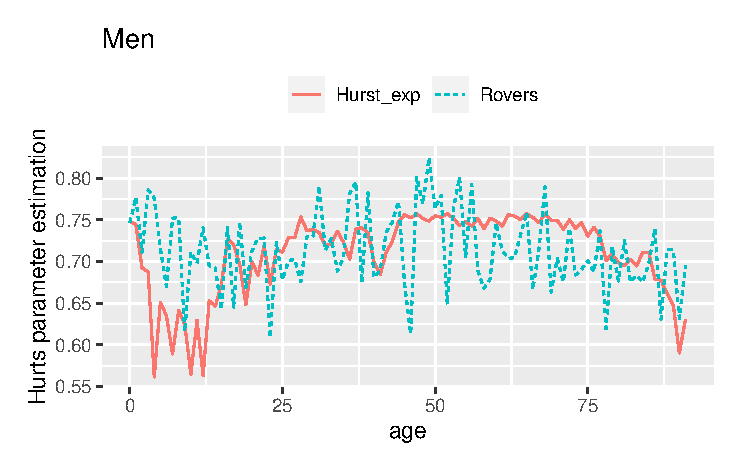
\includegraphics{Hurst-Men.eps}
        \caption{Estimated Hurst parameter using R - routines.}
    \end{figure}
    %
    \subsection{Results for women}
    \label{re-wom}

        We present the results for \num{10000} path simulations of the 
    mortality rates for ages: 
    $
        \num{0}, \num{5}, \num{25}, 
        \num{50},\num{60}, \num{70}, 
        \num{80},\num{90}
    $.
        We graph the historical mortality rate, the mean of all simulations and 
    the \num{95}\% confidence interval. See figures \ref{graph-simu_FOU1} and
    \ref{graph-simu_FOU2}.

        In general, for all ages, the model is well fitted, in particular,
    after the \num{80}'s. Nevertheless, there are some time periods where the 
    model is not so good as we want to. For instance, the model underestimates 
    the mortality rate for women age \num{0} during the period of 
    \num{50}s to \num{80}s and for women age \num{50}, \num{60},
    \num{80} and \num{90} during \num{60}s to \num{80}s approximately. 
    Moreover, it also overestimates the mortality rate for
    women age \num{25} during the period of \num{50}s to \num{80}s.

    \begin{figure}[H]
        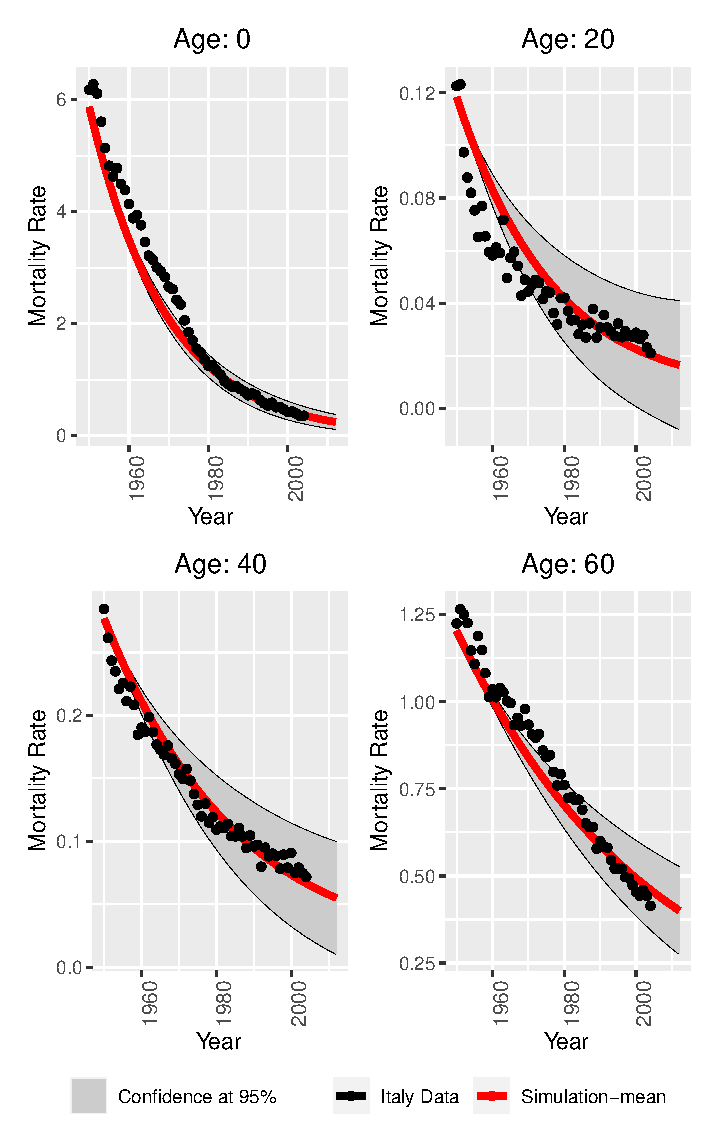
\includegraphics{woman_confidence_bands.eps}
         \caption{%
             Simulations for the rate mortality with the fOU model: ages
             \num{0}, num{20}, \num{40}, \num{60} and $N=\num{10000}$ simulation
             paths.
         }
             \label{graph-simu_FOU1}
    \end{figure}

    \begin{figure}[H]
        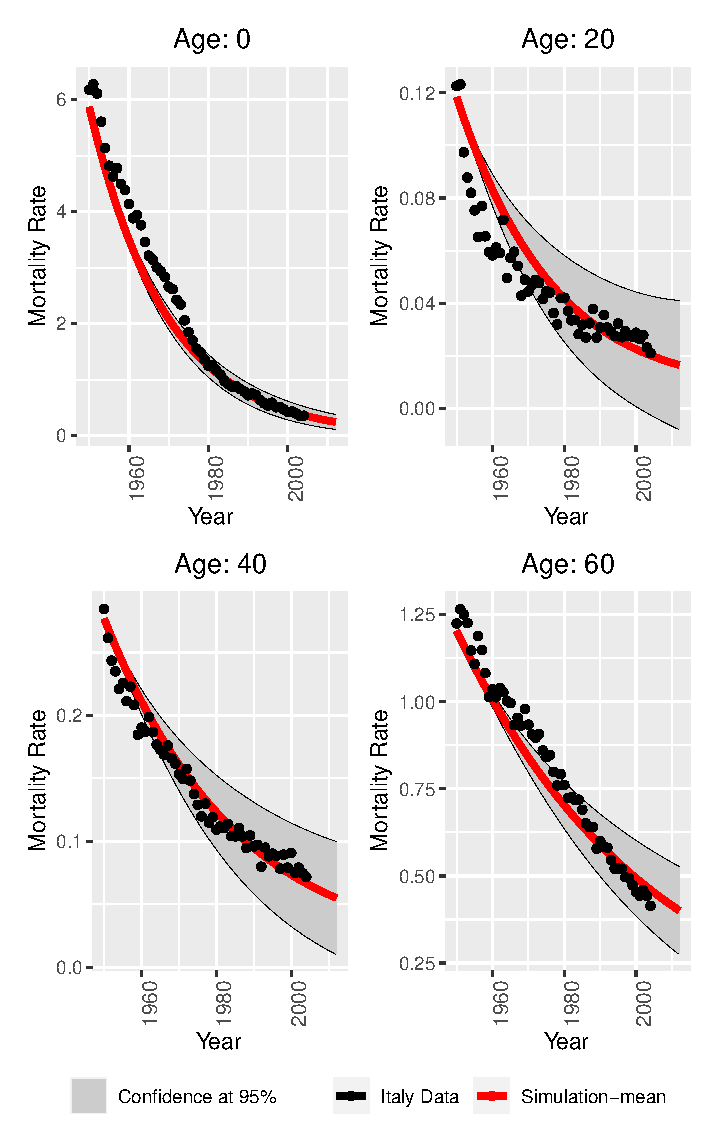
\includegraphics{man_confidence_bands.eps}
        \caption{%
            Simulations for the rate mortality with the fOU model: ages
            \num{0}, num{20}, \num{40}, \num{60} and $N=\num{10000}$ simulation
            paths.
        }
        \label{graph-simu_FOU1_}
    \end{figure}

        For older ages (see figure \ref{graph-simu_FOU2}) we observe that for 
    ages \num{60} and \num{70} the estimation is well fitted trough the years. 
    We notice that predicted rates are not so far away and that the historical 
    rates are inside the confidence interval. For the very oldest ages the 
    estimation is not so good as for earlier ages. The main difference is in 
    \num{50}'s when the absolute number of
    living persons arriving to those ages were small so that the variability of 
    the estimates is larger. 

        All these suggest that a better model could include a short and a 
    long-term memory process, so that the model could help us to control the 
    short-term variations in a better way.

    \subsection{Results for men}\label{re-men}

        As in the case for women, we present results for 10000 simulations of 
    the mortality rates for ages: 
    $
        \num{0}, 
        \num{5}, 
        \num{25}, 
        \num{50}, 
        \num{60}, 
        \num{70}, 
        \num{80}, 
        \num{90}
    $.
    We graph the historical rate mortality, the mean of all simulations and the
    \num{95.5}\% confidence interval. See figures \ref{graph-simu_FOU3} and
    \ref{graph-simu_FOU4}.

        As in the case for women, the proposed model for men is well fitted.
    We observe an increase in the rates mortality at ages between 25 to 35, this
    caused a overestimation in the first 35 years and latter a underestimation
    of the mortality rates. As was mentioned before, if we include in the model 
    a short-term process,  we believe the model could be better fitted. The main
    example  of a short-term process to try is a AR$(p)$ with $p\le 2$ or $3$.

        For older ages, we observed that the data is irregular, so it is 
    necessary to use a more complex model to
    fit this data.

\section{Forecast}

        When we use our model to forecast and compare with the real data 
    between the years \num{2005} to \num{2014}. In general, from our results we 
    observe that the forecast for women are good for almost all ages we tested. 
    For men the variability of the results is strong and the behavior of the
    forecast is in general not good as those for women; for instance for ages 
    smaller than 10 the results are quite similar than for women, even for ages 
    between \num{10} and \num{45} it is possible to
    consider the results just good. However, for ages greater than \num{50}, 
    the results are not good, in fact, for older ages the results are bad: the 
    model overstimate the mortality rates.

        We present the results in the figures 
    \ref{graph-graph-forecast_women_FOU1} for women at ages 
    $\num{0},
     \num{25},
     \num{50},
     \num{90}
    $. For men we present more ages to ilustrate that the
    results are bad as the ages increases. see figures
    \ref{graph-forecast_men_FOU1} and \ref{graph-forecast_men_FOU2} at ages
    $
        \num{0},
        \num{25},
        \num{50},
        \num{90}
    $.

%\begin{figure}[H]
%    \caption{Forecast for the rate mortality with the fOU model. Women at ages
%    $0,25,50,90$.}
%    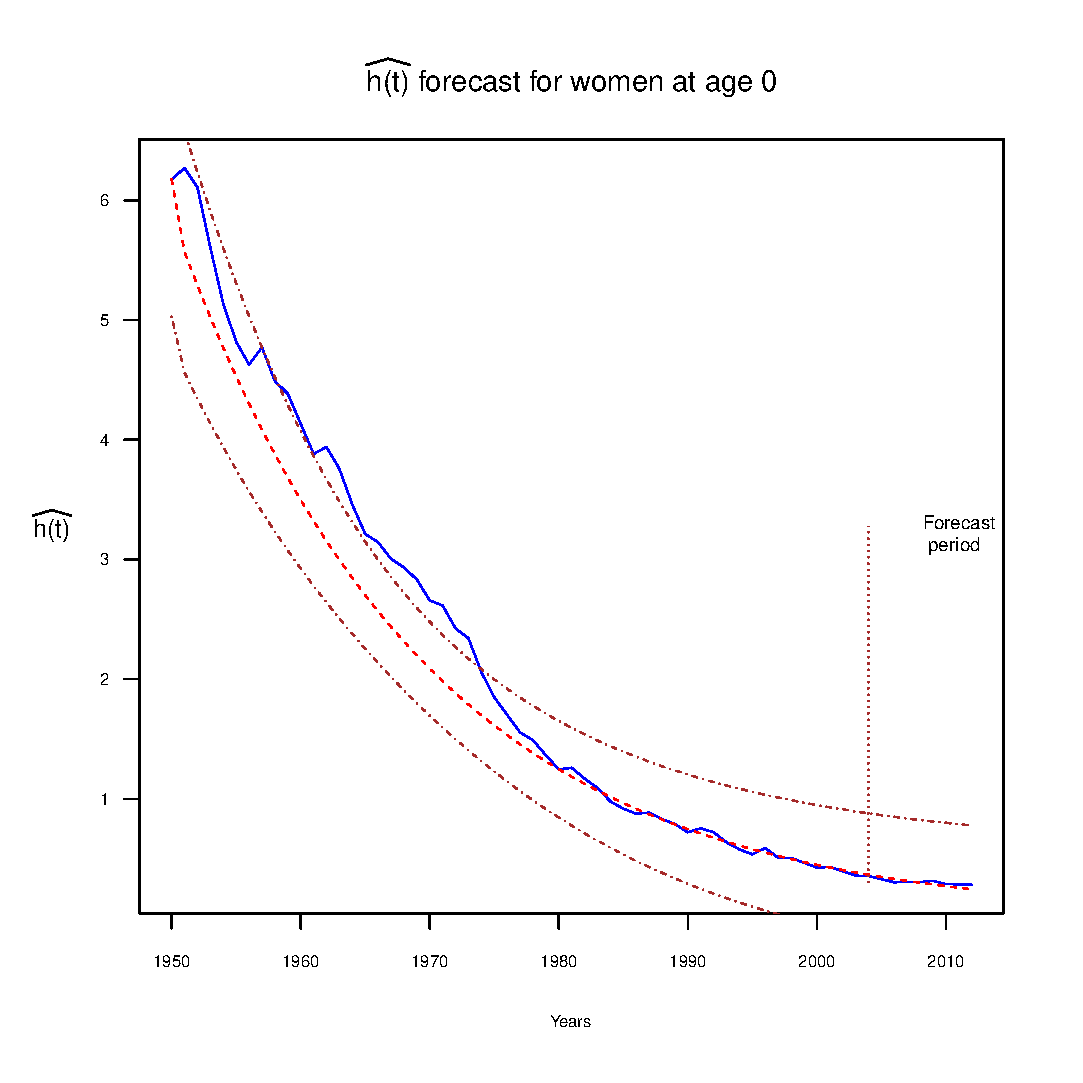
\includegraphics[width = 2.85in]{PlotWomenForecast0.eps}
%    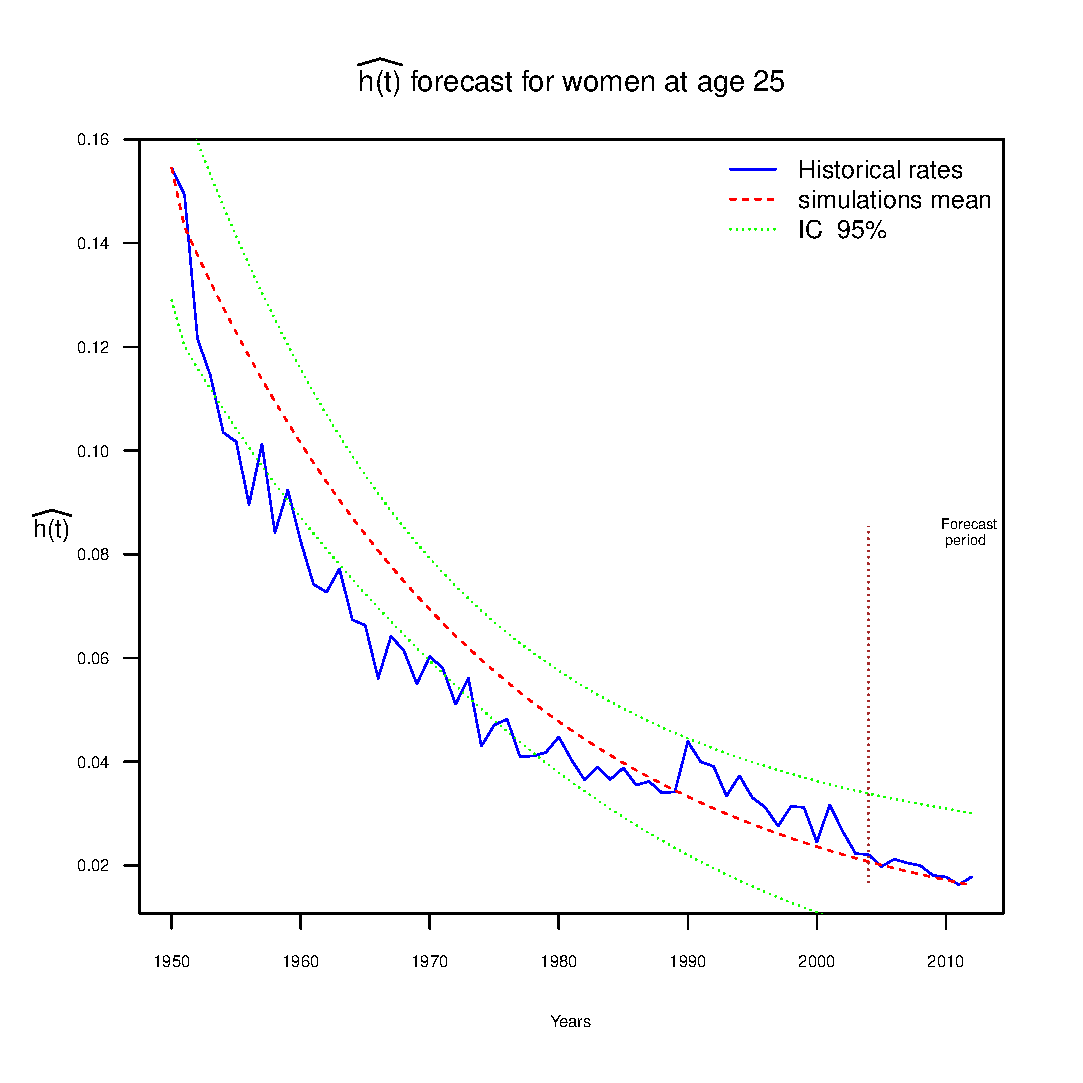
\includegraphics[width = 2.85in]{PlotWomenForecast25.eps}
%    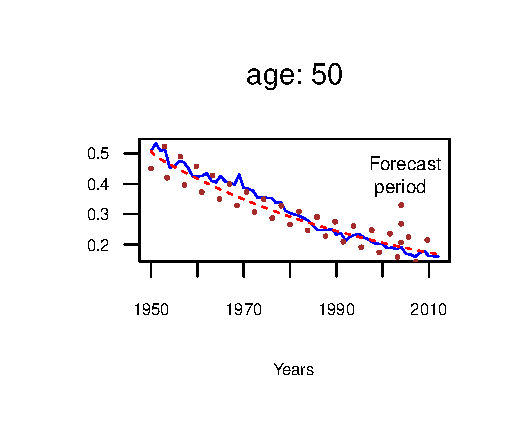
\includegraphics[width = 2.85in]{PlotWomenForecast50.eps}
%    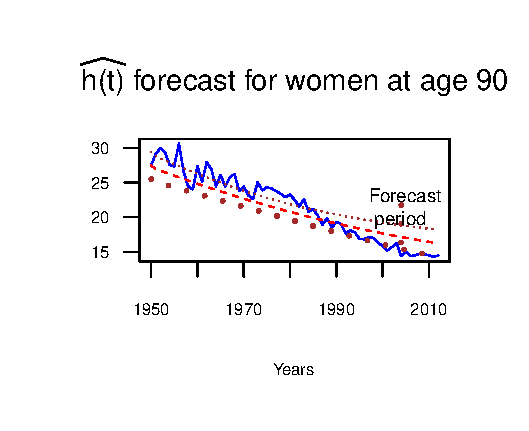
\includegraphics[width = 2.85in]{PlotWomenForecast90.eps}
%    \caption{
%        Forecast for the rate mortality with the fOU model. 
%        Women at ages $0,25,50,90$.
%        \qquad
%        {\protect
%            \tikz
%            \protect
%            \draw[dotted, color=brown, style={line width=1pt}] 
%            plot coordinates{(0.0cm, 0.0cm) (.2cm, 0.2cm)};
%        }
%        IC at 95\% 
%        \qquad
%        {\protect
%            \tikz
%            \protect
%            \draw[dashed, color=red, style={line width=1pt}] 
%            plot coordinates{(0,0) (.2cm, 0.2cm)};
%        }
%        simulation mean
%        \qquad
%        {\protect
%            \tikz
%            \protect
%            \draw[solid, color=blue, style={line width=1pt}] 
%            plot coordinates{(0,0) (.2cm, 0.2)};
%        }
%        Data mortality rates.
%    }
%    \label{graph-graph-forecast_women_FOU1}
%\end{figure}\vspace*{0.1cm}

%\begin{figure}[H]
%    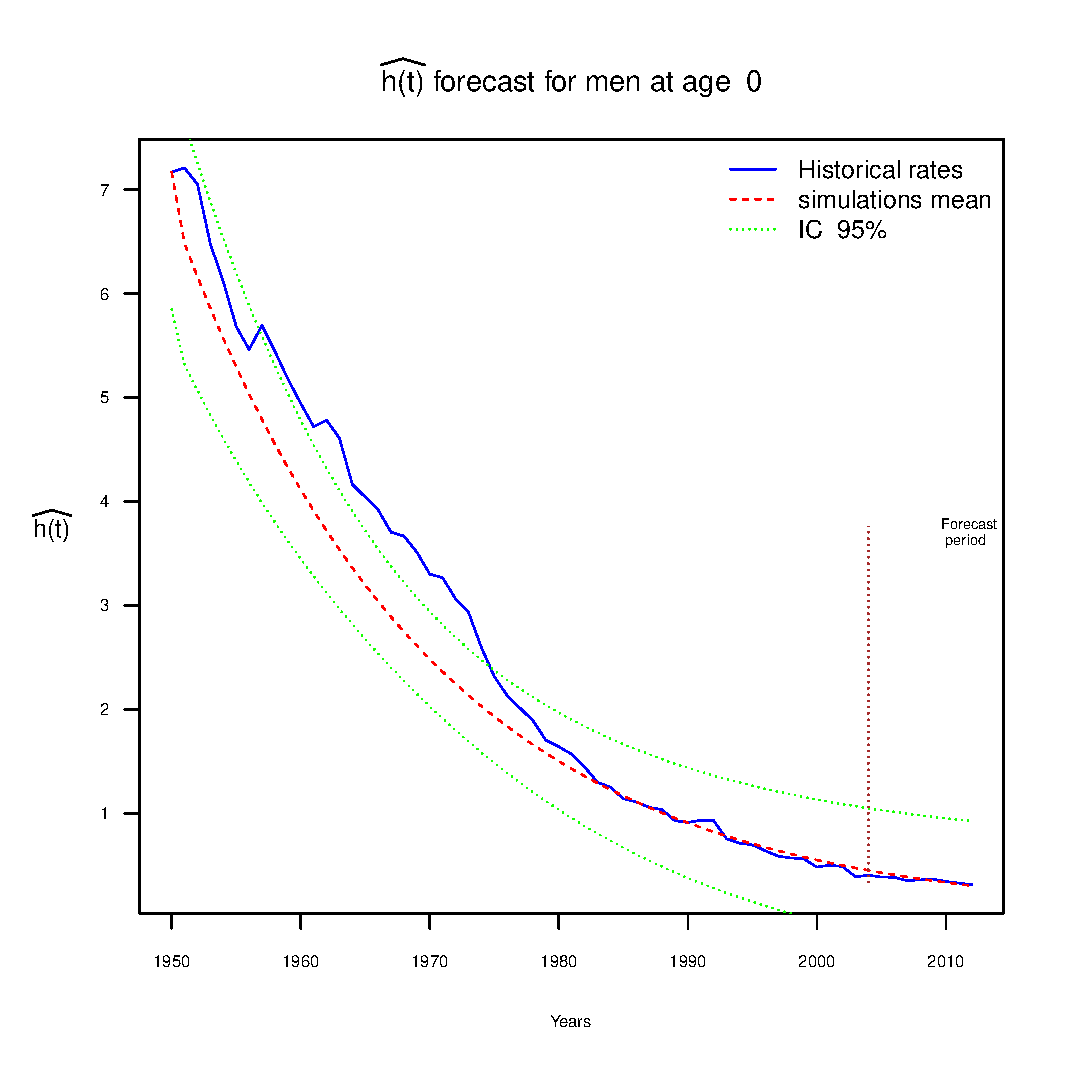
\includegraphics[width = 2.85in]{PlotMenForecast0.eps}
%    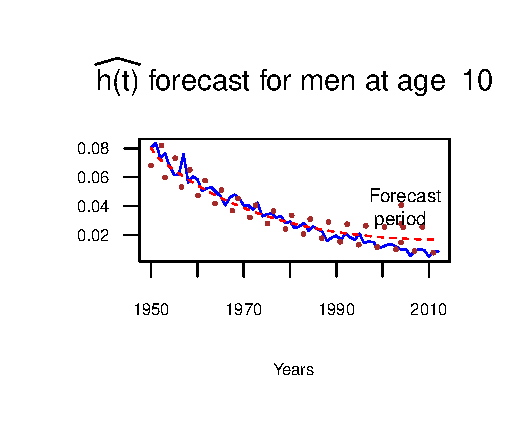
\includegraphics[width = 2.85in]{PlotMenForecast10.eps}
%    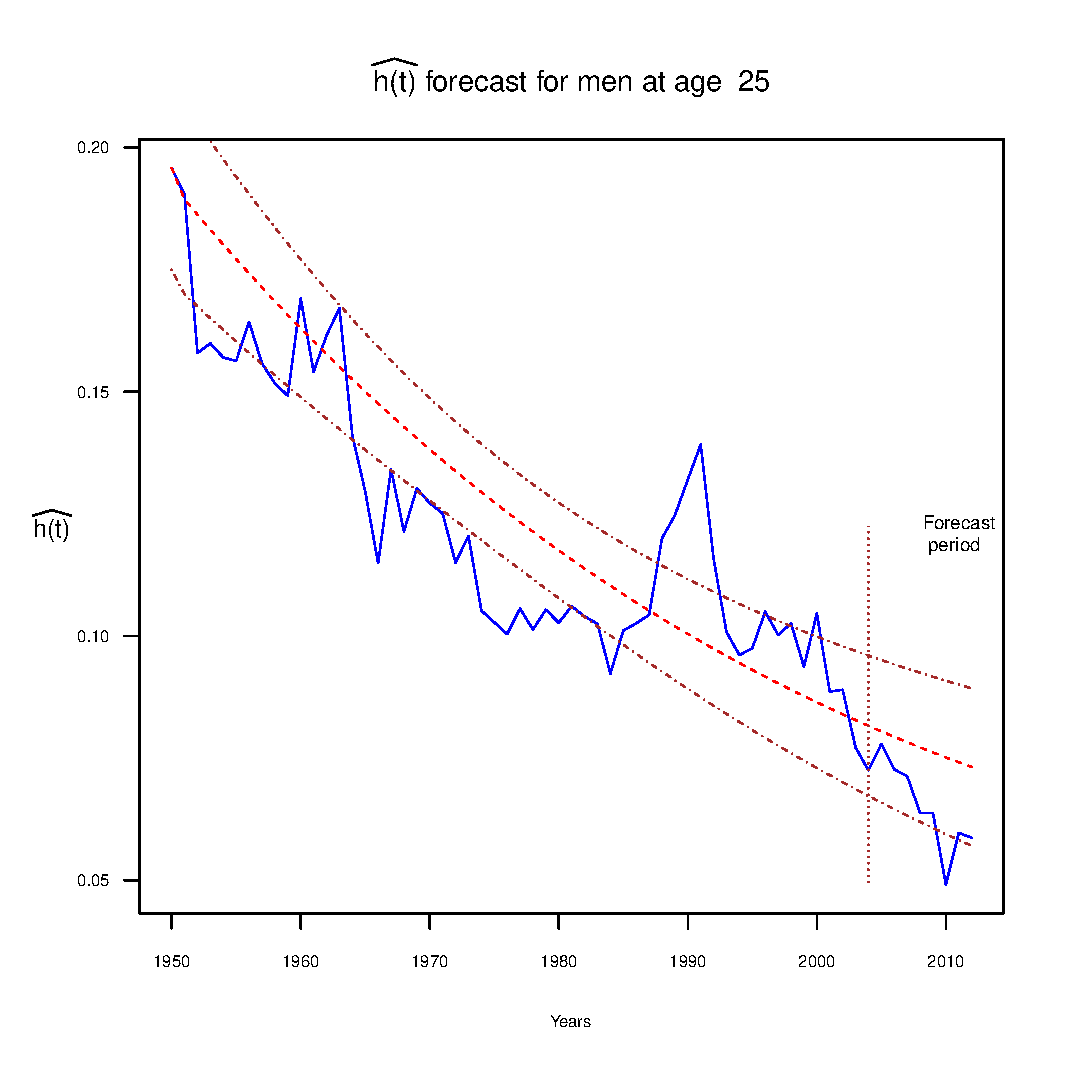
\includegraphics[width = 2.85in]{PlotMenForecast25.eps}
%    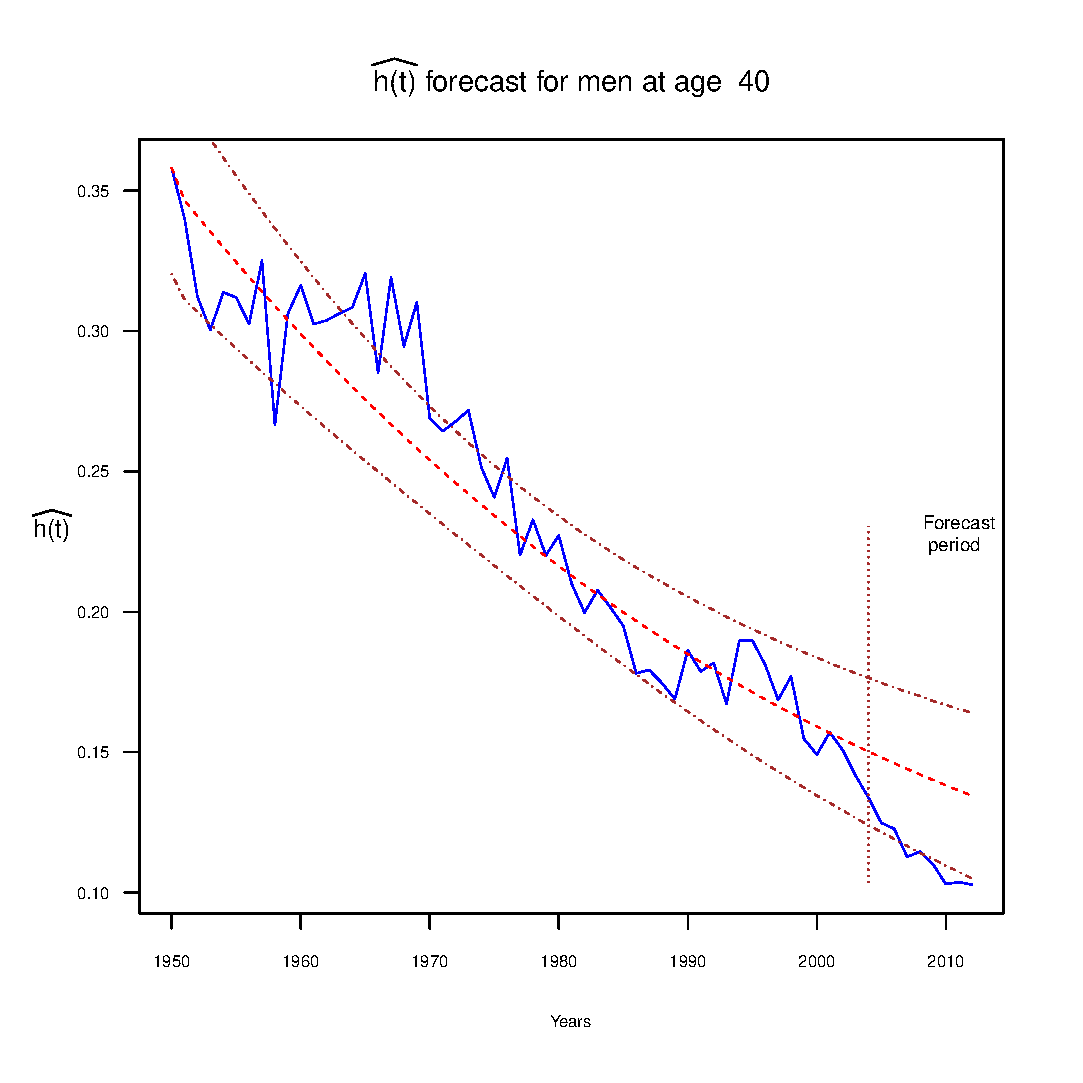
\includegraphics[width = 2.85in]{PlotMenForecast40.eps}
%    \label{graph-forecast_men_FOU1}
%    \caption{
%        Forecast for the rate mortality with the fOU model. Men 
%        at ages $0,10,25,40$.
%        \newline
%        \qquad
%        {\protect
%            \tikz
%            \protect
%            \draw[dotted, color=brown, style={line width=1pt}] 
%            plot coordinates{(0.0cm, 0.0cm) (.2cm, 0.2cm)};
%        }
%        IC at 95\% 
%        \qquad
%        {\protect
%            \tikz
%            \protect
%            \draw[dashed, color=red, style={line width=1pt}] 
%            plot coordinates{(0,0) (.2cm, 0.2cm)};
%        }
%        simulation mean
%        \qquad
%        {\protect
%            \tikz
%            \protect
%            \draw[solid, color=blue, style={line width=1pt}] 
%            plot coordinates{(0,0) (.2cm, 0.2)};
%        }
%        Data mortality rates.
%    }
%\end{figure}

%\begin{figure}[H]
%
%    \caption{Forecast for the rate mortality with the fOU model. Men at ages
%    $50,60,70,90$.}
%    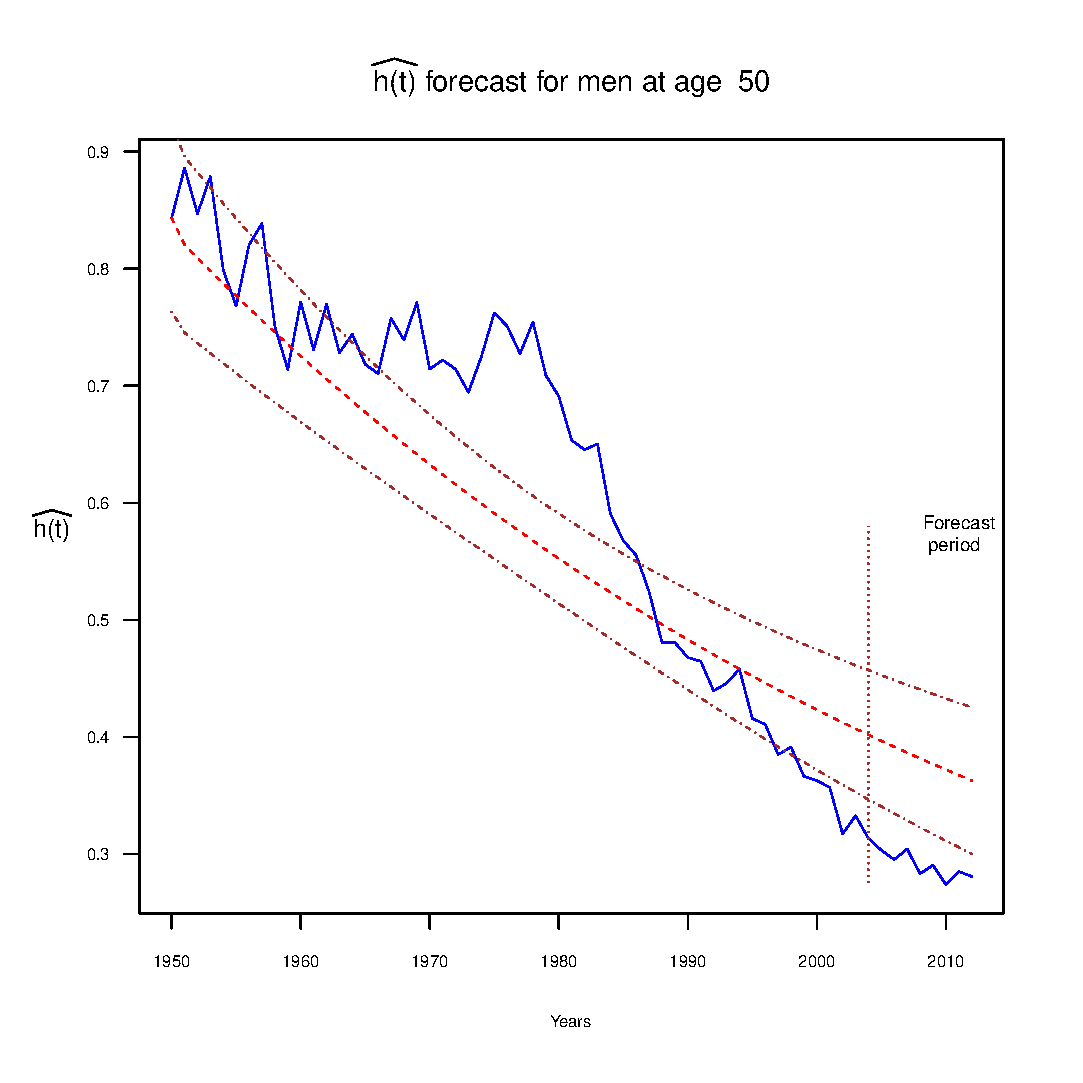
\includegraphics[width = 2.85in]{PlotMenForecast50.eps}
%    \includegraphics[width = 2.85in]{PlotMenForecast60.eps}
%    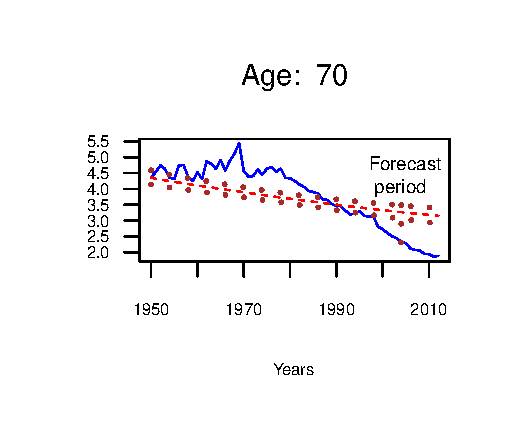
\includegraphics[width = 2.85in]{PlotMenForecast70.eps}
%    \includegraphics[width = 2.85in]{PlotMenForecast90.eps}
%    \caption{Forecast for the rate mortality with the fOU model. 
%        Men at ages $50,60,70,90$.
%        \newline
%        \qquad
%        {\protect
%            \tikz
%            \protect
%            \draw[dotted, color=brown, style={line width=1pt}] 
%            plot coordinates{(0.0cm, 0.0cm) (.2cm, 0.2cm)};
%        }
%        IC at 95\% 
%        \qquad
%        {\protect
%            \tikz
%            \protect
%            \draw[dashed, color=red, style={line width=1pt}] 
%            plot coordinates{(0,0) (.2cm, 0.2cm)};
%        }
%        simulation mean
%        \qquad
%        {\protect
%            \tikz
%            \protect
%            \draw[solid, color=blue, style={line width=1pt}] 
%            plot coordinates{(0,0) (.2cm, 0.2)};
%        }
%        Data mortality rates.
%}
%    \label{graph-forecast_men_FOU2}
%\end{figure}\vspace*{0.1cm}


\section{Conclusions}\label{sec:Conclutions}

        We have applied our proposed model to the Italian mortality rates with a
    geometric-type fractional Ornstein-Uhlenbeck process. Our main hypothesis 
    was that, for a fixed age, the mortality rates changes through the time 
    slowly, so that a stochastic differential equations that captures the 
    long-range dependence  could be a good model. We have used a stochastic 
    differential equation with a fractional Brownian motion as a driven noise 
    with $H \in (\num{0.5}, \num{1})$ in order to satisfy the long-range 
    dependence property. With the data we have fixed the Hurst coefficient and 
    we have confirmed our hypothesis since we have found that the estimated 
    Hurst, for all ages, is in 
    $
        (
            \num{0.58},
            \num{0.8}
        )
    $.  

        Notice that we have consider a more general model that the one used in
    \cite{gi-or-be}. This is because we have included the possibility that the
    Hurst parameter could be equal to $1/2$, which is the case when the 
    fractional Brownian motion becomes a standard Brownian motion. Therefore,
    when $H=1/2$ we recover the  Giacometti, Ortobelli and Bertocchi model.

        % FGN with  single parameter $H$ is a simplified model of reality. 
    %Therefore,
    % it may be not appropriate for some phenomena, even though it is much more
    %consistent with reality than the AR and ARMA process.
    % A generalized and comprehensive family of processes, which can include a
    %larger number of parameters and incorporates both the
    % FGN and the ARMA processes, has been studied by Koutsoyiannis \cite{kou}. 
    % One
    %possible generalization
    % of the ARMA process is the FARIMA process, which is a long memory process
    % (see, for instance, section 5.2 in \cite{sh-st}).

        The model is, specially for women, well behaved. For men at some ages 
    we found some shortcomings that suggest the use of more terms in order to 
    improve the model. From this results, and in opposition of the European 
    normative on insurance  that does not discriminate by gender, we conclude 
    from our model, applied  to the Italian case, that modelling the mortality 
    by gender could improve  the risk management of the insurance companies.

        The long-range dependence model proposed in this paper is good
    enough to reproduce the mortality rates. If we add some extra terms to make 
    it more flexible to reproduce the cases where the mortality rates have more
    variations then it will generate a more accurate model. We are starting to 
    work on this extension of the model. Moreover, a multiplicative noise model 
    will be the subject of a future research.

    \bibliography{references.bib}{}
\end{document}
